\documentclass[border=10pt]{standalone}
\usepackage{pgfplots}
\usepgfplotslibrary{colormaps}
\pgfplotsset{compat=1.18}

\begin{document}
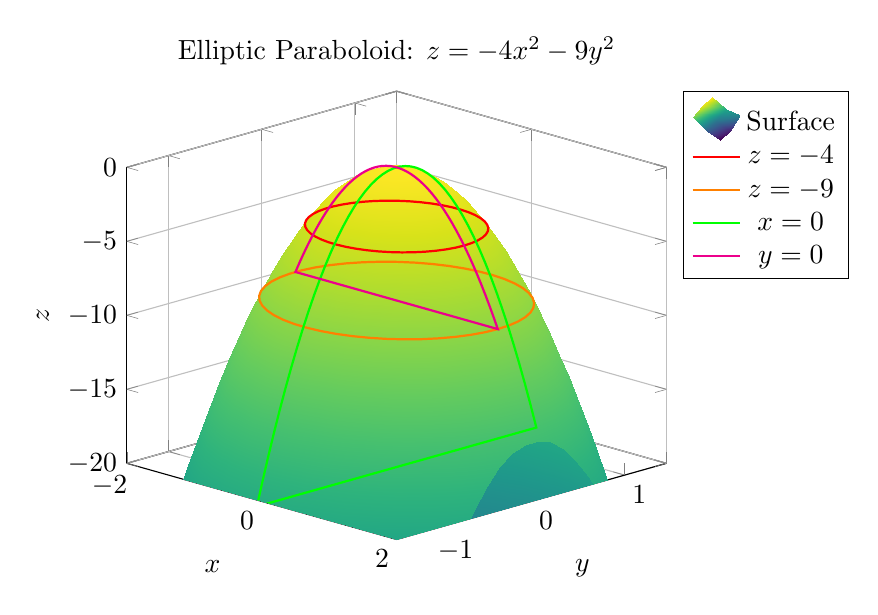
\begin{tikzpicture}
\begin{axis}[
    view={45}{20},
    xlabel={$x$},
    ylabel={$y$},
    zlabel={$z$},
    title={Elliptic Paraboloid: $z = -4x^2 - 9y^2$},
    colormap/viridis,
    domain=-2:2,
    y domain=-2:2,
    samples=30,
    zmin=-20,
    zmax=0,
    enlargelimits=false,
    grid=major,
    legend pos=outer north east,
]
% Main surface
\addplot3[surf, shader=interp] {-4*x^2 - 9*y^2};

% Horizontal trace at z = -4 (ellipse)
\addplot3[domain=0:360, samples=50, thick, red] ({cos(\x)}, {(2/3)*sin(\x)}, {-4});

% Horizontal trace at z = -9 (ellipse)
\addplot3[domain=0:360, samples=50, thick, orange] ({1.5*cos(\x)}, {sin(\x)}, {-9});

% Vertical trace at x = 0 (parabola)
\addplot3[domain=-1.5:1.5, samples=50, thick, green] ({0}, {x}, {-9*x^2});

% Vertical trace at y = 0 (parabola)
\addplot3[domain=-1.5:1.5, samples=50, thick, magenta] ({x}, {0}, {-4*x^2});

\legend{Surface, $z=-4$, $z=-9$, $x=0$, $y=0$}
\end{axis}
\end{tikzpicture}
\end{document}
